\documentclass[addpoints,12pt]{exam}
\usepackage[utf8]{inputenc}
\usepackage[spanish,es-noshorthands]{babel}
\usepackage{amsmath,amssymb}
\usepackage{graphicx}
\usepackage{array}
\usepackage{xcolor}
\usepackage{tikz}
\usetikzlibrary{calc,arrows.meta,decorations.markings}
\usepackage[most]{tcolorbox}
\usepackage[legalpaper,margin=2cm,top=1.8cm]{geometry}

\graphicspath{{./}}

% ---- estilos tikz para la figura del cuarto de anillo + varilla ----
\tikzset{
  ejeflecha/.style = {->, black, thick},
  guia/.style      = {black, dashed, thin},
  dim/.style       = {<->, black, thin}
}

% ---- encabezado de pregunta: numero + caja de puntaje en linea con el texto ----
\qformat{}
\newcommand{\qpts}[1]{{\setlength{\fboxsep}{2.5pt}\fbox{#1}}\hspace{0.6em}\ignorespaces}
\newcommand{\qhead}[1]{\thequestion.\hspace{0.5em}\qpts{#1}}
\newcommand{\pts}[1]{\textcolor{red}{\textbf{(#1 pts)}}}

% ---- encabezado / pie (clase exam) ----
\pagestyle{headandfoot}
\runningheadrule
\firstpageheader{}{}{}
\runningheader{\small F\'isica II - Electromagnetismo}%
              {\small\textbf{Certamen 1}}%
              {\small 31 de Agosto, 2026}
\firstpagefooter{}{\thepage}{}
\runningfooter{}{Page \thepage\ of \numpages}{}

\begin{document}

%========================================================
% PORTADA
%========================================================
\begin{center}
    
\includegraphics[height=1.9cm]{logo ubb.png}\hspace{1cm}%
    
\includegraphics[height=1.5cm]{logo dfis.png}\\[0.5cm]
    {\Large F\'isica II - Electromagnetismo}\\[0.15cm]
    {\LARGE\textbf{Certamen 1}}\\[0.9cm]
    31 de Agosto, 2026
\end{center}

\vspace{0.7cm}

\noindent\textbf{Nombre}: \hrulefill\\[0.7cm]
\noindent\textbf{Rut}: \makebox[6.5cm]{\hrulefill}\hspace{0.3cm}\textbf{Folio}: \hrulefill

\vspace{0.4cm}
\noindent\rule{\textwidth}{1pt}
\vspace{0.2cm}

\noindent\textbf{Algunas consideraciones para esta evaluaci\'on:}
\begin{itemize}\setlength\itemsep{2pt}
    \item El certamen 1 contiene 5 p\'aginas (incluida la portada) y 3 preguntas, con un total de
          59 puntos.
    \item Cada pregunta debe ser respondida por s\'olo una respuesta. En caso de presentar m\'as de
          una, se anulan las respuestas.
    \item \textbf{No est\'a permitido el uso de celulares o tablet en el desarrollo de esta
          evaluaci\'on. De ser sorprendido utilizando estos art\'iculos su evaluaci\'on ser\'a
          calificada con nota 1.0.}
    \item Buena suerte!
\end{itemize}

\noindent Seleccione con una \textbf{X} el nombre del profesor de su secci\'on:

\vspace{0.15cm}
\noindent
\begin{minipage}{0.49\textwidth}
\begin{tabular}{|l|p{1.1cm}|}
\hline
Prof.\ Evelyn Riveros & \\ \hline
Prof.\ Mor\'in \'Ordenes & \\ \hline
Prof.\ Luis Soto & \\ \hline
\end{tabular}
\end{minipage}%
\begin{minipage}{0.49\textwidth}
\begin{tabular}{|l|p{1.1cm}|}
\hline
Prof.\ Luis Liempi & \\ \hline
Prof.\ Diego Ram\'irez & \\ \hline
Prof.\ Arturo Fern\'andez & \\ \hline
\end{tabular}
\end{minipage}

\vspace{0.9cm}
\begin{center}
{\large\textbf{Puntaje}}\\[0.2cm]
\gradetable[v][questions]
\end{center}

\newpage

%========================================================
% PREGUNTAS
%========================================================
\begin{questions}

%--------------------------------------------------------
% PREGUNTA 1  (Forma Normal: esferas 1A)
%--------------------------------------------------------
\question[20]
\begin{minipage}[t]{0.56\textwidth}
\vspace{0pt}
\qhead{20}Tres esferas peque\~nas pintadas de distintos colores se encuentran cargadas, ubicadas
seg\'un el sistema de referencia de la figura:
\smallskip

\noindent$\bullet$~Esfera \textbf{verde}: $q_V=-86{,}8\,\mu$C, en $X=4{,}00$ cm, $Y=6{,}00$ cm.\\
$\bullet$~Esfera \textbf{azul}: $q_A=16{,}0\,\mu$C, en $R=6{,}00$ cm, $\theta=30{,}0^\circ$.\\
$\bullet$~Esfera \textbf{roja}: $q_R=169\,\mu$C, en $X=0$ cm, $Y=3{,}00$ cm.
\end{minipage}\hfill
\begin{minipage}[t]{0.40\textwidth}
\vspace{0pt}
\centering
\begin{tikzpicture}[scale=0.48, >=Stealth, line width=0.7pt]
    \draw[->,gray] (-1.5,0)--(7.6,0) node[right,font=\scriptsize]{$x$ [cm]};
    \draw[->,gray] (0,-1)--(0,7.6) node[above,font=\scriptsize]{$y$ [cm]};
    \node[gray,font=\tiny,below left] at (0,0){$O$};
    \draw[dashed,gray] (0,0)--(5.196,3);
    \draw (1.4,0) arc (0:30:1.4);
    \node[font=\tiny] at (2.05,0.5){$30^\circ$};
    \filldraw[green!55!black] (4,6) circle (7pt);
    \node[green!55!black,above,font=\scriptsize] at (4,6.6){verde};
    \filldraw[blue] (5.196,3) circle (7pt);
    \node[blue,right,font=\scriptsize] at (5.5,3){azul};
    \filldraw[red] (0,3) circle (7pt);
    \node[red,left,font=\scriptsize] at (-0.35,3){roja};
\end{tikzpicture}\\[2pt]
{\footnotesize Fig.\ 1}
\end{minipage}

\smallskip
\noindent\textbf{(a)} Calcule la fuerza el\'ectrica que ejerce la esfera azul sobre la esfera roja. \pts{8}

\vspace{7cm}
\noindent\textbf{(b)} Calcule la fuerza el\'ectrica que ejerce la esfera verde sobre la esfera roja. \pts{8}

\vspace{7cm}
\noindent\textbf{(c)} Calcule la fuerza el\'ectrica resultante sobre la esfera roja. \pts{4}

\newpage

%--------------------------------------------------------
% PREGUNTA 2  (Forma Normal: circulo Version 1)
%--------------------------------------------------------
\question[19]
\begin{minipage}[t]{0.56\textwidth}
\vspace{0pt}
\qhead{19}Considere una circunferencia de radio $20$ cm, en la cual se encuentra un sistema de dos
cargas el\'ectricas, como se muestra en la figura. Las cargas tienen valores $q_1=12\,\mu$C y
$q_2=-6\,\mu$C.

\smallskip
\noindent\textbf{(a)} Dibuje y represente el vector campo el\'ectrico producido por cada una de las
cargas en los puntos $P_1$ y $P_2$, identificando cada vector seg\'un la carga que lo genera
(dib\'ujelos sobre la figura). \pts{4}
\end{minipage}\hfill
\begin{minipage}[t]{0.40\textwidth}
\vspace{0pt}
\centering
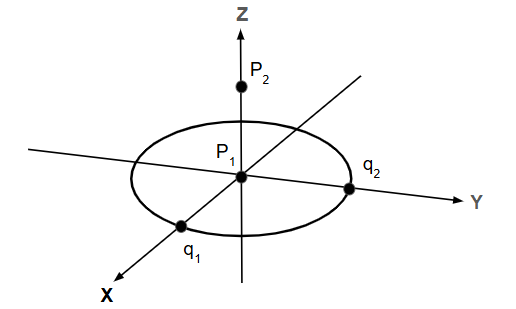
\includegraphics[width=\textwidth]{fig_q2_v1.png}\\[2pt]
{\footnotesize Fig.\ 2}
\end{minipage}

\vspace{0.4cm}
\noindent\textbf{(b)} Determine el campo el\'ectrico neto generado por el sistema de cargas en el punto
$P_1$, ubicado en el origen del sistema de coordenadas. \pts{7}

\vspace{10cm}
\noindent\textbf{(c)} Determine el campo el\'ectrico neto generado por el sistema de cargas en el punto
$P_2$, ubicado $30$ cm sobre el centro de la circunferencia. \pts{8}

\newpage

%--------------------------------------------------------
% PREGUNTA 3  (Forma Normal: cuarto de anillo + varilla, Version 1)
%--------------------------------------------------------
\question[20]
\begin{minipage}[t]{0.58\textwidth}
\vspace{0pt}
\qhead{20}En el plano $xy$ se tiene un cuarto de anillo de radio $R=0{,}5$ m, centrado en el origen $O$
y ubicado en el primer cuadrante, con densidad de carga lineal uniforme $\lambda_1=6$ nC/m. Sobre el
eje $+y$, desde $y=R$ hasta $y=5R$, se encuentra una varilla cargada uniformemente, cuya carga total es
$Q_2=-4$ nC. Ambas distribuciones de carga se muestran en la figura. Determine:

\smallskip
\noindent\textbf{(a)} La carga total $Q_1$ del cuarto de anillo. \pts{2}
\end{minipage}\hfill
\begin{minipage}[t]{0.38\textwidth}
\vspace{0pt}
\centering
\begin{tikzpicture}[>=Stealth, thick, scale=0.72]
  \coordinate (O) at (0,0);
  \draw[ejeflecha] (-0.8,0) -- (3.2,0) node[right, font=\scriptsize]{$x^+$};
  \draw[ejeflecha] (0,-0.8) -- (0,7.2) node[right, font=\scriptsize]{$y^+$};
  \draw[line width=1.6pt, black!80] (2,0) arc[start angle=0, end angle=90, radius=2];
  \foreach \ang in {12,30,48,66,84}{\node[font=\scriptsize] at (\ang:2.15){$+$};}
  \node[font=\small] at (1.7,1.9){$\lambda_1$};
  \draw[line width=2.6pt, black!70] (0,2) -- (0,6.5);
  \foreach \y in {2.4,2.95,3.5,4.05,4.6,5.15,5.7,6.25}{\node[font=\scriptsize] at (0.2,\y){$-$};}
  \node[font=\small] at (0.7,4.25){$\lambda_2$};
  \node[font=\normalsize\bfseries, above left=1pt] at (O){$O$};
  \draw[dim] (-0.6,0) -- (-0.6,2) node[midway, left, font=\small]{$R$};
  \draw[black, thin] (-0.45,0)--(-0.75,0);
  \draw[black, thin] (-0.45,2)--(-0.75,2);
  \draw[dim] (-1.1,2) -- (-1.1,6.5) node[midway, left, font=\small]{$4R$};
  \draw[black, thin] (-0.95,2)--(-1.25,2);
  \draw[black, thin] (-0.95,6.5)--(-1.25,6.5);
\end{tikzpicture}\\[2pt]
{\footnotesize Fig.\ 3}
\end{minipage}

\vspace{0.7cm}
\noindent\textbf{(b)} La densidad lineal de carga $\lambda_2$ de la varilla. \pts{2}

\vspace{1.7cm}
\noindent\textbf{(c)} El campo el\'ectrico en el origen generado por el cuarto de anillo. \pts{8}

\vspace{7.5cm}
\noindent\textbf{(d)} El campo el\'ectrico en el origen generado por la varilla. \pts{8}

\end{questions}

\newpage

%========================================================
% FORMULARIO
%========================================================
\newtcolorbox{formbox}[1]{colback=gray!3, colframe=gray!55, coltitle=white,
    colbacktitle=gray!45, fonttitle=\bfseries, boxrule=0.5pt, arc=2pt,
    left=6pt,right=6pt,top=2pt,bottom=2pt, before skip=4pt, after skip=4pt,
    title={#1}}
\setlength{\jot}{2pt}

\begin{formbox}{Ley de Coulomb (forma vectorial)}
\[
    \vec{F}_{12} = k_e\,\frac{q_1 q_2}{|\vec{r}_1 - \vec{r}_2|^{3}}\,(\vec{r}_1 - \vec{r}_2),
    \qquad k_e = 9\times10^{9}\ \mathrm{N\,m^2/C^2}
\]
\end{formbox}

\begin{formbox}{Campo el\'ectrico de una carga puntual}
\[
    \vec{E} = k_e\,\frac{q}{|\vec{r}_p - \vec{r}_q|^{3}}\,(\vec{r}_p - \vec{r}_q)
\]
\end{formbox}

\begin{formbox}{Campo el\'ectrico debido a una distribuci\'on continua}
\[
    \vec{E} = k_e \int \frac{dq}{|\vec{r}_p - \vec{r}_q|^{3}}\,(\vec{r}_p - \vec{r}_q)
\]
\end{formbox}

\begin{formbox}{Densidad lineal de carga}
\[
    \lambda = \frac{dq}{dl} \qquad\Longrightarrow\qquad dq = \lambda\,dl
\]
\end{formbox}

\begin{formbox}{Ejemplos de integrales t\'ipicas en electrost\'atica}
\noindent
\begin{minipage}{0.52\textwidth}
\begin{itemize}\setlength\itemsep{1pt}
    \item $\displaystyle\int \frac{x\,dx}{(a^2 + x^2)^{3/2}} = -\frac{1}{\sqrt{x^2 + a^2}} + C$
    \item $\displaystyle\int \frac{dx}{\sqrt{a^2 + x^2}} = \ln\left|x + \sqrt{x^2 + a^2}\right| + C$
    \item $\displaystyle\int \frac{1}{r^2}\,dr = -\frac{1}{r} + C$
    \item $\displaystyle\int \frac{dx}{(x^2 + a^2)^{3/2}} = \frac{x}{a^2\sqrt{x^2 + a^2}}$
\end{itemize}
\end{minipage}%
\begin{minipage}{0.46\textwidth}
\begin{itemize}\setlength\itemsep{1pt}
    \item $\displaystyle\int_0^{2\pi} d\theta = 2\pi$
    \item $\displaystyle\int \cos\theta\,d\theta = \sin\theta + C$
    \item $\displaystyle\int \sin\theta\,d\theta = -\cos\theta + C$
    \item $\displaystyle\int r^n\,dr = \frac{r^{n+1}}{n+1}$
\end{itemize}
\end{minipage}
\end{formbox}

\begin{formbox}{Prefijos}
$c=10^{-2}$, \quad $m=10^{-3}$, \quad $\mu=10^{-6}$, \quad $n=10^{-9}$, \quad $p=10^{-12}$.
\end{formbox}

\end{document}
